% --------------------------------------------------
% Literature Review
% --------------------------------------------------
% The literature review is an essential component of your project report. You should discuss the existing literature that is relevant to your project with full and proper referencing. You should aim to refer to a range of material including academic papers, text books, articles and existing product descriptions. It should be clear to the reader why the literature you identify is relevant and how you have incorporated the learnings from your review into your project. For example, you may have made a number of project 
% Page 4 of 5 decisions based on your review of the literature and these decisions should be described. The literature review should also lead to the creation of a number of possible solutions to your problem articulation and technical specification

\chapter{Literature Review} \label{lit}

This chapter focuses on an analysis of existing systems in the online development space and the literature that provides context to the decisions that were made during development. It looks at the advancement of the web browser and discusses the functionality provided which can lead to this type of project to be developed. It also looks at the current state of the art of virtualization as it relates to personalised environments and how the advent of Containers has fundamentally changed the way users interact with virtual environments, as illustrated by supporting literature.

%TODO: This might be a waste of space?
\section{The Web Browser} \label{lit-web}

The web browser has been through a myriad of changes since it's birth in the early 1990s. An excellent article titled "Mosaic and the World-Wide-Web"\cite{mosaic} illustrates the problems that were prominent in the early stages of the industry such as the lack of a search engine leading to difficulty in finding resources. It also illustrates what were considered leaps in progress at the time such as Mosaic being the first browser to support in-line multimedia and to have a 'back' and 'forward' button.

Such concepts that were developed during the time are still very relevant, the general TCP/IP stack had been determined and the HTTP protocol was in use. An issue with HTTP is the protocol by design has latency embedded as it is designed for sending structured messages. For a project attempting to create an environment that mirrors a local set up online latency is a big hurdle and the need for it to be real-time is key. 

\section{Real-Time Communication} \label{lit-web}

An experiment was done in 2012 discussing the performance of different RTC methods by Professors at the University of New Brunswick\cite{websocket}.

\textbf{HTTP polling} is an attempt to solve the real-time issue however it is still built on top of a system not designed for real-time, full duplex communication. \textbf{HTTP long-polling} is another solution that sticks to the HTTP protocol but reduces the number of wasteful requests by having the server intelligently not respond to the request if there is no information available and hang until a timeout or information becomes available.

A modern solution to this is the \textbf{WebSocket} protocol proposed in RFC 6455 \cite{wsrfc} which aims to reduce latency by a factor of 3 compared to HTTP in the real-time communication aspect. It is a fully duplexed, bidirectional communication channel that uses physical sockets to connect machines.

%TODO: Illustration of WebSocket vs HTTP

\section{Online Developer Environments} \label{lit-ode}

A number of existing solutions providing online development environments exist and have been analysed for the purpose of this review.

\subsection{Repl.it}

Repl.it is very similar to the idea proposed in the Problem Statement (Section \ref{section:probart-probstate}) and a lot of the requirements lined out in Section \ref{section:probart-techspec}. It offers a huge array of Repl templates available for users to get started with many languages/frameworks very quickly. It also uses the Monaco Editor provided by Microsoft in order to provide a first class text editor experience.

Repl.it takes advantage of containerisation in order to gives users the full developer experience when visiting the system \cite{replit-containers}. The system also uses it's own container orchestration software in order to scale the instances available to users up and down depending on demand.

Every code result that is available to be viewed/run is viewable through a special .repl.run subdomain. This includes long running processes like web servers which are able to be hosted from these subdomains and be always accessible. This means you could create several repls which all connect to each other like a full system.

Technically the system is very impressive, something that the system doesn't recreate quite as smoothly as a local environment would is a small amount of latency between a key being pressed and the corresponding value appearing in the REPL itself.

The system also seems to remove all previously typed entries of the REPL on every press of the \textit{Run} button. This suggests that it is giving you a new REPL instance on every execution which isn't how a local environment works.

From a HCI point of view the website feels very smooth to use and is not frustrating to use other than the latency noted when typing directly into the running container via the REPL.

Repl.it is clearly very focused on the objective of replacing local development environments and does a good job of fulfilling that need.

\subsection{Codecademy}
Codecademy is a educational focused online environment designed to teach users how to code. Ranging in topics from beginning web development to a course to the IBM Watson API. It is a more directed experience than Repl.it as users are performing tasks for exercises but they are typing code into a similar environment, the code is executed and the result is displayed to the user.

Codecademy does allow access directly to the REPL but if code is entered into the editor which allows for user input such as the \texttt{input()} function in Python. Then it interprets the input correctly.

The Codecademy web application is clearly a very complicated system and it shows by how unresponsive it feels when navigating from page to page. The page does a full refresh even though there are elements which do not change on the screen page to page. This leads to a frustrating wait looking a blank screen between page loads.

It is clear that Codecademy is a focused environment to encourage new developers to get into development by offering an easy to start environment and heavily directed experience. It is not concerned with the idea of replacing local development environments so much as making sure that it's not something beginners should need to think of when wanted to get to know a new tool.

\subsection{Glitch}
Glitch is a web application that is focused on trying to cultivate a social coding community that encourages developers to help each other out and build mini applications with JavaScript and Node.js. It provides an online coding environment that uses containers to isolate the users runtime.

Glitch is clearly focused heavily on the social aspect as on the homepage they have a section dedicated to users asking for help so more experienced coders can help them achieve their goals with the applications they want to build. It also showcases user made projects on the homepage which can be \textit{Remixed} which is similar to forking a repository on GitHub for other users to modify.

In terms of design, the website has a very colourful friendly interface. A feature which is particularly notable is in each project editor there is an option to view \textit{Container Stats} where the CPU usage in \%, Memory usage in bytes and additional relevant information can be found. There is also guidelines on the technical restrictions to projects that are run in Glitch. 


%TODO: Finish section
\section{Virtual Machines and Containers} \label{lit-containers}

\subsection{Virtual Machines}

Virtualisation is a technique in computing that, most commonly, is seen by users in the \textbf{Virtual Machine} \textit{(VM)} software. Virtual Machines are heavily utilised to provide virtual desktop environments on top of a users already existing desktop. The advantages of which are a sandbox environment for potentially harmful operations, such as when penetration testers are trying to fingerprint a virus. The option of trying a different OS without needing to dedicate a partition of disk space to it or deal with a dual booting set up is another user facing benefit of virtual machines.

In the enterprise world, Virtual Machines are being used to host their customers applications in a full PaaS solution so customers no longer have to worry about hosting their own web servers or other online services.

The general way of interacting with fully virtualised environments is through a hypervisor which is a tool that is responsible for provisioning and monitoring Virtual Machines \cite{hypervisor}. The hypervisor allocates resources such as memory and CPU cores from the host machine that the VM is allowed to consume. When the VM is shut down these resources are freed and can be used by the host system once again. The hypervisor also allows the VM to use a different base operating system than the one that is on the host machine as it provides a whole \textit{Guest OS}.

\subsection{Containers}

Containers are a much lighter virtualisation method than  Virtual Machines despite the functionality being similar. They achieve this as they are much closer to the systems 'bare metal' as any commands that are executed through a container are running on the host's hardware. This means that there is no need for a hypervisor as containers have direct access to the resources. Usage limits can be set in the configuration of container \textit{images} which will be discussed further during this subsection.

As Containers traditionally don't utilise a hypervisor the biggest difference between them is that the engine that powers the container provisioning software such as the \textit{Docker Engine} isn't able to virtualise an environment based on a different OS. This is more by design however as it is what gives containers their 'light weight' quality as they aren't having to simulate a whole kernel.

\begin{figure}[h!]
    \centering
    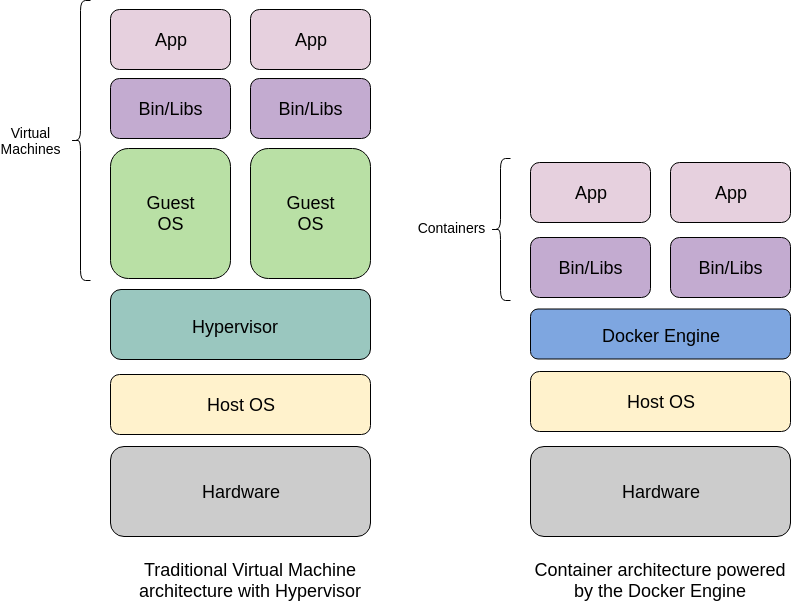
\includegraphics[scale=0.4]{res/Virtualisation.png}
    \caption{Architecture of Virtual Machines vs. Containers}
    \label{fig:architecture}
\end{figure}

https://ieeexplore.ieee.org/abstract/document/6903537

^^ Talking about containers vs VMs for PaaS software

https://ieeexplore.ieee.org/abstract/document/7158965

^^ More focused on Docker

\pagebreak
